\documentclass[11pt,a4paper]{article}
\usepackage[margin=22mm]{geometry}
\usepackage{fontspec}
\setmainfont{Latin Modern Roman}
\setsansfont{Latin Modern Sans}
\setmonofont{Latin Modern Mono}
\usepackage{amsmath,amssymb}
\usepackage{unicode-math}
\setmathfont{Latin Modern Math}
\usepackage{longtable,array,fvextra,adjustbox,needspace}
\usepackage{pgfplots}
\usepackage{pdflscape}
\pgfplotsset{compat=1.18}
\usepackage[colorlinks=true,linkcolor=blue,urlcolor=blue,unicode=true]{hyperref}
\usepackage{xurl}
\newcounter{listing}
\newcounter{scripttable}
\definecolor{pcd1}{HTML}{005A78}
\definecolor{pcd2}{HTML}{6B2CB1}
\definecolor{pcd3}{HTML}{447766}
\definecolor{pcd4}{HTML}{9A3E20}
\definecolor{pcd5}{HTML}{756000}
\setlength{\parindent}{0pt}
\setlength{\parskip}{0.65em}
\setlength{\emergencystretch}{3em}
\begin{document}
\hypersetup{pdftitle={Variables connect chemical questions with observations},pdfsubject={Authored thematic script},pdfcreator={Project Chemie Digital LaTeX exporter}}
\title{Variables connect chemical questions with observations}
\author{}
\date{}
\maketitle
\tableofcontents
\clearpage
\section{Give every observed value a variable, unit and role}
A variable identifies a property that can take different values. An observation records a value of that property for a specified object or occasion. In a calibration, concentration and absorbance are different variables; a prepared standard has a concentration, and an instrument reading supplies an observed absorbance. Their units and roles make the relationship interpretable.


The dilution series in \hyperref[material-dbd925a0d8ec6e2c6e4be6395abc9163339481c371aa49329875b23e9d743d4b]{Fig.~\ref*{material-dbd925a0d8ec6e2c6e4be6395abc9163339481c371aa49329875b23e9d743d4b}} gives this distinction a chemical setting. Preparing standards establishes a planned set of concentrations. Measuring them adds instrument responses. The table in \hyperref[material-f1b327d73189f443f14267bee0cf01025fc8215d6ba420873f334a4ee88fbd08]{Table~\ref*{material-f1b327d73189f443f14267bee0cf01025fc8215d6ba420873f334a4ee88fbd08}} keeps the controlled concentrations, observed responses and observation identities connected. These roles determine which quantity a calibration model will use to explain or predict another quantity.


\par\medskip
\Needspace{10cm}
\refstepcounter{figure}\label{material-dbd925a0d8ec6e2c6e4be6395abc9163339481c371aa49329875b23e9d743d4b}
\noindent\textbf{Fig.~\ref*{material-dbd925a0d8ec6e2c6e4be6395abc9163339481c371aa49329875b23e9d743d4b}.} UV/Vis dilution series: prepared concentration levels provide the controlled values for the calibration measurements.\par\nopagebreak
\begin{center}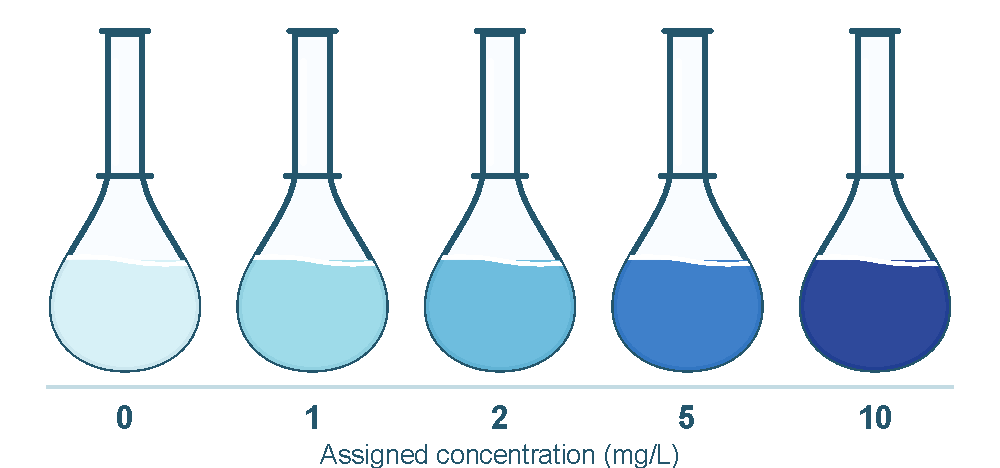
\includegraphics[width=\linewidth,height=.62\textheight,keepaspectratio]{asset-8590fa68e15cc53a13bf45173a518f07849ff7ea3bfd0453729713eeefcfc118.pdf}\end{center}

\medskip

\par\medskip
\Needspace{8\baselineskip}
\refstepcounter{scripttable}\label{material-f1b327d73189f443f14267bee0cf01025fc8215d6ba420873f334a4ee88fbd08}
\noindent\textbf{Table~\ref*{material-f1b327d73189f443f14267bee0cf01025fc8215d6ba420873f334a4ee88fbd08}.} Calibration observations with explicit roles for standard identity, concentration and measured absorbance.\par\nopagebreak
\begin{longtable}{@{}p{\dimexpr0.500000\linewidth-2\tabcolsep\relax}p{\dimexpr0.500000\linewidth-2\tabcolsep\relax}@{}}
Concentration (mg/L) & Absorbance \\ \hline
\endhead
0 & 0.031 \\ \hline
1 & 0.105 \\ \hline
2 & 0.182 \\ \hline
5 & 0.406 \\ \hline
10 & 0.779 \\ \hline
\end{longtable}
\medskip

The response plot in \hyperref[material-1fb414fe87569aa1e766560525239098111745ddbe04cbb06618dc0b0a912190]{Fig.~\ref*{material-1fb414fe87569aa1e766560525239098111745ddbe04cbb06618dc0b0a912190}} then displays the relationship between the two numerical variables. Reading the axes is the first interpretation step: each point represents an observation with a concentration coordinate and an absorbance coordinate. A model can summarize the pattern while repeated readings reveal how much response varies at a given concentration.


\par\medskip
\Needspace{10cm}
\refstepcounter{figure}\label{material-1fb414fe87569aa1e766560525239098111745ddbe04cbb06618dc0b0a912190}
\noindent\textbf{Fig.~\ref*{material-1fb414fe87569aa1e766560525239098111745ddbe04cbb06618dc0b0a912190}.} Observed absorbance against prepared concentration in the UV/Vis calibration example. The point coordinates pair the two variables for each observation.\par\nopagebreak
\begin{center}
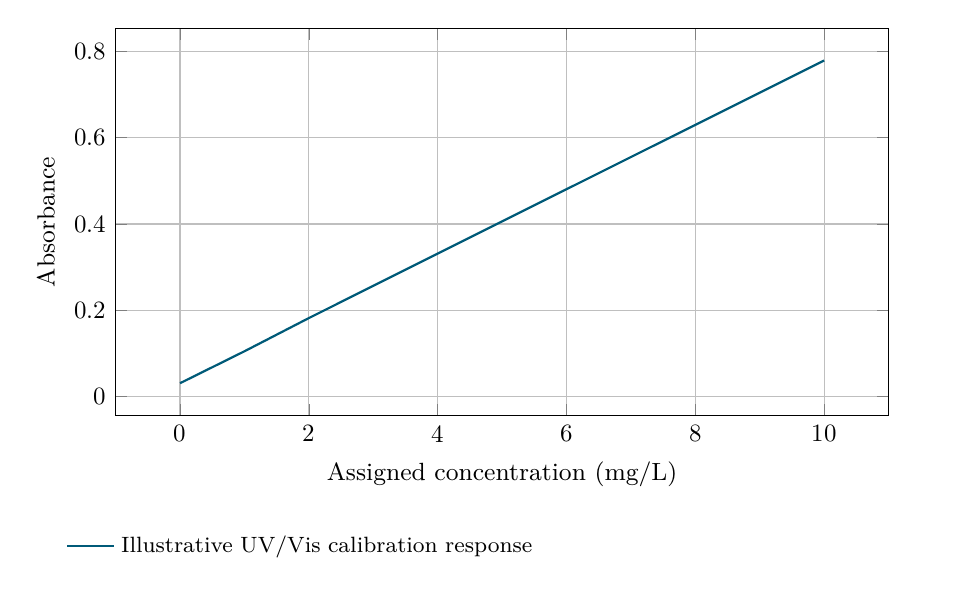
\begin{tikzpicture}
\begin{axis}[width=0.94\linewidth,
height=6.5cm,
scale only axis=false,
grid=major,
tick label style={font=\small},
label style={font=\small},
xlabel={Assigned concentration (mg/L)},
ylabel={Absorbance},
legend style={font=\footnotesize,draw=none,at={(0.5,-0.28)},anchor=north,legend columns=1,text width=0.85\linewidth,align=left},
unbounded coords=jump,
scaled ticks=false]
\addplot[color=pcd1,thick,mark=none] coordinates {(0,0.031) (1,0.105) (2,0.182) (5,0.406) (10,0.779)};
\addlegendentry{Illustrative UV/Vis calibration response}

\end{axis}
\end{tikzpicture}
\end{center}

\medskip

\clearpage
\section{The repeated unit determines which variation is observed}
A lake study adds a second level of organization. A sampling site identifies where water was collected, while a repeated reading identifies a measurement of that collected material. The map in \hyperref[material-820aea9ff3cdbde1a101fe1c07e1c99120fc1a9f0db965493c1bba81dd391578]{Fig.~\ref*{material-820aea9ff3cdbde1a101fe1c07e1c99120fc1a9f0db965493c1bba81dd391578}} establishes the spatial setting; the observation table in \hyperref[material-24ba92170e3477b37dff328c5a24efce2430b0fe52efc690d8bc736c54321918]{Table~\ref*{material-24ba92170e3477b37dff328c5a24efce2430b0fe52efc690d8bc736c54321918}} retains the site and replicate grouping.


\par\medskip
\Needspace{10cm}
\refstepcounter{figure}\label{material-820aea9ff3cdbde1a101fe1c07e1c99120fc1a9f0db965493c1bba81dd391578}
\noindent\textbf{Fig.~\ref*{material-820aea9ff3cdbde1a101fe1c07e1c99120fc1a9f0db965493c1bba81dd391578}.} Lake sampling locations used to identify the spatial origin of the analyte observations.\par\nopagebreak
\begin{center}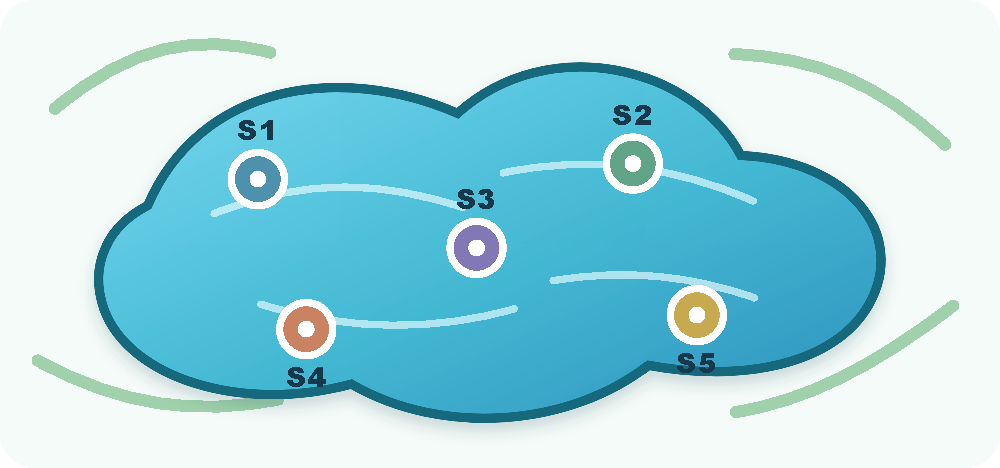
\includegraphics[width=\linewidth,height=.62\textheight,keepaspectratio]{asset-35377bf4fc7c155621091d8914a23a4ee2819e9d3490b535aa3d4faa4b7d44c4.pdf}\end{center}

\medskip

\par\medskip
\Needspace{8\baselineskip}
\refstepcounter{scripttable}\label{material-24ba92170e3477b37dff328c5a24efce2430b0fe52efc690d8bc736c54321918}
\noindent\textbf{Table~\ref*{material-24ba92170e3477b37dff328c5a24efce2430b0fe52efc690d8bc736c54321918}.} Analyte A observations grouped by lake site and measurement replicate, preserving the authored units and values.\par\nopagebreak
\begin{longtable}{@{}p{\dimexpr0.250000\linewidth-2\tabcolsep\relax}p{\dimexpr0.250000\linewidth-2\tabcolsep\relax}p{\dimexpr0.250000\linewidth-2\tabcolsep\relax}p{\dimexpr0.250000\linewidth-2\tabcolsep\relax}@{}}
Sampling site & Replicate 1 & Replicate 2 & Replicate 3 \\ \hline
\endhead
Site 1 & 5.02 & 4.96 & 5.05 \\ \hline
Site 2 & 4.98 & 5.01 & 4.95 \\ \hline
Site 3 & 5.04 & 5.00 & 4.97 \\ \hline
Site 4 & 4.99 & 5.03 & 5.01 \\ \hline
Site 5 & 4.96 & 5.02 & 4.98 \\ \hline
\end{longtable}
\medskip

The grouped plot in \hyperref[material-0a4621dfcf71259b699eee1c96f50fe772410435e5f10259a78ae068274c9851]{Fig.~\ref*{material-0a4621dfcf71259b699eee1c96f50fe772410435e5f10259a78ae068274c9851}} lets us compare variation within sites with differences between sites. Repeated instrument readings characterize the part of the procedure that was repeated. Collecting independent water samples additionally represents sampling variation. A design that repeats both stages allows their contributions to be studied separately.


\par\medskip
\Needspace{10cm}
\refstepcounter{figure}\label{material-0a4621dfcf71259b699eee1c96f50fe772410435e5f10259a78ae068274c9851}
\noindent\textbf{Fig.~\ref*{material-0a4621dfcf71259b699eee1c96f50fe772410435e5f10259a78ae068274c9851}.} Analyte A replicate results grouped by sampling site. Within-site spread and between-site location are read at their respective design levels.\par\nopagebreak
\begin{center}
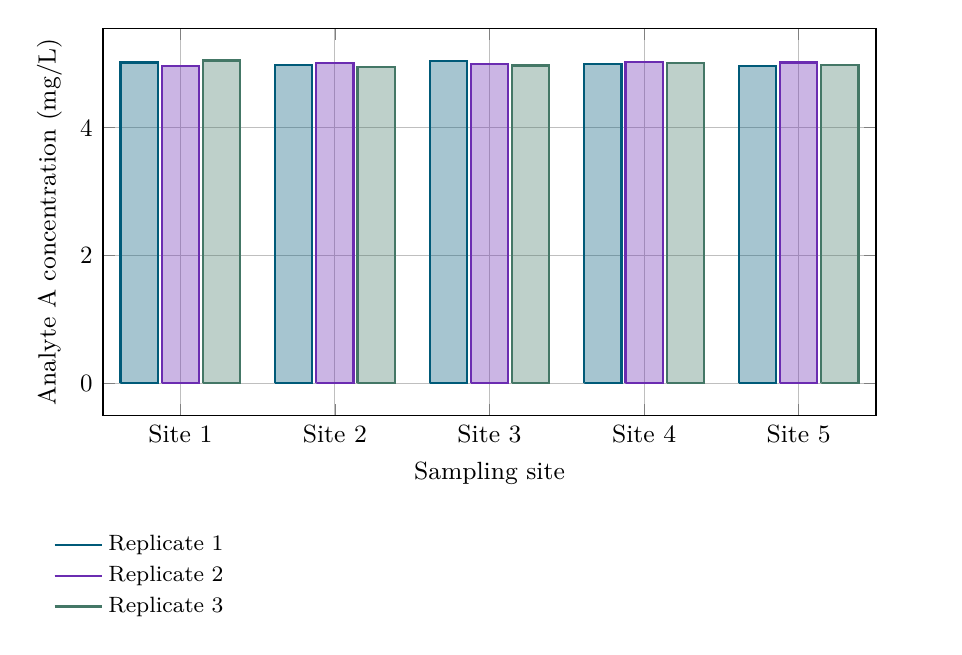
\begin{tikzpicture}
\begin{axis}[width=0.94\linewidth,
height=6.5cm,
scale only axis=false,
grid=major,
tick label style={font=\small},
label style={font=\small},
xlabel={Sampling site},
ylabel={Analyte A concentration (mg/L)},
legend style={font=\footnotesize,draw=none,at={(0.5,-0.28)},anchor=north,legend columns=1,text width=0.85\linewidth,align=left},
unbounded coords=jump,
scaled ticks=false,
xmin=0.5,
xmax=5.5,
xtick={1,2,3,4,5},
xticklabels={{Site 1},{Site 2},{Site 3},{Site 4},{Site 5}}]
\addplot[color=pcd1,thick,fill=pcd1,fill opacity=0.35,mark=none] coordinates {(0.6133333333333334,0) (0.6133333333333334,5.02) (0.8533333333333334,5.02) (0.8533333333333334,0)} \closedcycle;
\addplot[color=pcd1,thick,fill=pcd1,fill opacity=0.35,forget plot,mark=none] coordinates {(1.6133333333333333,0) (1.6133333333333333,4.98) (1.8533333333333335,4.98) (1.8533333333333335,0)} \closedcycle;
\addplot[color=pcd1,thick,fill=pcd1,fill opacity=0.35,forget plot,mark=none] coordinates {(2.6133333333333333,0) (2.6133333333333333,5.04) (2.8533333333333335,5.04) (2.8533333333333335,0)} \closedcycle;
\addplot[color=pcd1,thick,fill=pcd1,fill opacity=0.35,forget plot,mark=none] coordinates {(3.6133333333333333,0) (3.6133333333333333,4.99) (3.8533333333333335,4.99) (3.8533333333333335,0)} \closedcycle;
\addplot[color=pcd1,thick,fill=pcd1,fill opacity=0.35,forget plot,mark=none] coordinates {(4.613333333333333,0) (4.613333333333333,4.96) (4.8533333333333335,4.96) (4.8533333333333335,0)} \closedcycle;
\addlegendentry{Replicate 1}
\addplot[color=pcd2,thick,fill=pcd2,fill opacity=0.35,mark=none] coordinates {(0.88,0) (0.88,4.96) (1.12,4.96) (1.12,0)} \closedcycle;
\addplot[color=pcd2,thick,fill=pcd2,fill opacity=0.35,forget plot,mark=none] coordinates {(1.88,0) (1.88,5.01) (2.12,5.01) (2.12,0)} \closedcycle;
\addplot[color=pcd2,thick,fill=pcd2,fill opacity=0.35,forget plot,mark=none] coordinates {(2.88,0) (2.88,5) (3.12,5) (3.12,0)} \closedcycle;
\addplot[color=pcd2,thick,fill=pcd2,fill opacity=0.35,forget plot,mark=none] coordinates {(3.88,0) (3.88,5.03) (4.12,5.03) (4.12,0)} \closedcycle;
\addplot[color=pcd2,thick,fill=pcd2,fill opacity=0.35,forget plot,mark=none] coordinates {(4.88,0) (4.88,5.02) (5.12,5.02) (5.12,0)} \closedcycle;
\addlegendentry{Replicate 2}
\addplot[color=pcd3,thick,fill=pcd3,fill opacity=0.35,mark=none] coordinates {(1.1466666666666665,0) (1.1466666666666665,5.05) (1.3866666666666667,5.05) (1.3866666666666667,0)} \closedcycle;
\addplot[color=pcd3,thick,fill=pcd3,fill opacity=0.35,forget plot,mark=none] coordinates {(2.1466666666666665,0) (2.1466666666666665,4.95) (2.3866666666666667,4.95) (2.3866666666666667,0)} \closedcycle;
\addplot[color=pcd3,thick,fill=pcd3,fill opacity=0.35,forget plot,mark=none] coordinates {(3.1466666666666665,0) (3.1466666666666665,4.97) (3.3866666666666667,4.97) (3.3866666666666667,0)} \closedcycle;
\addplot[color=pcd3,thick,fill=pcd3,fill opacity=0.35,forget plot,mark=none] coordinates {(4.1466666666666665,0) (4.1466666666666665,5.01) (4.386666666666667,5.01) (4.386666666666667,0)} \closedcycle;
\addplot[color=pcd3,thick,fill=pcd3,fill opacity=0.35,forget plot,mark=none] coordinates {(5.1466666666666665,0) (5.1466666666666665,4.98) (5.386666666666667,4.98) (5.386666666666667,0)} \closedcycle;
\addlegendentry{Replicate 3}

\end{axis}
\end{tikzpicture}
\end{center}

\medskip

This reasoning also applies inside an instrument. The variation-source diagram in \hyperref[material-1d3e62c8511295f2c7c4af782e59a475039c8f4da5db119df65562319d7d30b9]{Fig.~\ref*{material-1d3e62c8511295f2c7c4af782e59a475039c8f4da5db119df65562319d7d30b9}} organizes contributions along the UV/Vis measurement process. Preparation, measurement conditions and electronics can each affect the response. Identifying those stages helps us choose what to hold stable, what to vary deliberately and what to record as context for interpretation.


\par\medskip
\Needspace{10cm}
\refstepcounter{figure}\label{material-1d3e62c8511295f2c7c4af782e59a475039c8f4da5db119df65562319d7d30b9}
\noindent\textbf{Fig.~\ref*{material-1d3e62c8511295f2c7c4af782e59a475039c8f4da5db119df65562319d7d30b9}.} Sources of response variation along the UV/Vis measurement process, with the authored process stages retained.\par\nopagebreak
\par\medskip\noindent\textcolor{pcd1}{\textbf{1. DESIGNED INPUT}}\quad c\ensuremath{{}_i}\par
We choose the nominal concentration.

\par\noindent $\longrightarrow$ 2. input
\par\medskip\noindent\textcolor{pcd2}{\textbf{2. PROCESS}}\par
Chemical and analytical process

\par\noindent $\longrightarrow$ 3. produces
\par\noindent $\longrightarrow$ 4. affected by
\par\medskip\noindent\textcolor{pcd3}{\textbf{3. OBSERVED OUTPUT}}\quad A\ensuremath{{}_i}\par
We measure the absorbance.


\par\medskip\noindent\textcolor{pcd4}{\textbf{4. ADDITIONAL INFLUENCES}}\par

\par\textbf{PREPARATION} Pipetting, handling
\par\textbf{CONDITIONS} Temperature, timing
\par\textbf{MEASUREMENT} Noise, instrument drift
\par\noindent $\longrightarrow$ 5. combined residual
\par\medskip\noindent\textcolor{pcd5}{\textbf{5. COMBINED UNEXPLAINED EFFECTS}}\quad \ensuremath{\varepsilon}\ensuremath{{}_i}\par



\medskip

\clearpage
\section{Separate the systematic response from remaining variation}
A response model describes how an observed signal relates to explanatory quantities under stated conditions. In the additive UV/Vis model (\hyperref[material-7ee5e00a122e5d332a15d266d57783a4b2f1db7c6b22da0aeddaff32ce94398b]{Eq.~\ref*{material-7ee5e00a122e5d332a15d266d57783a4b2f1db7c6b22da0aeddaff32ce94398b}}), the systematic concentration-dependent contribution and the remaining contribution together describe the measured response. The attached symbol legend states the role and unit of every term.


\par\medskip
\begin{samepage}
\refstepcounter{equation}\label{material-7ee5e00a122e5d332a15d266d57783a4b2f1db7c6b22da0aeddaff32ce94398b}
\noindent\textbf{Eq.~\ref*{material-7ee5e00a122e5d332a15d266d57783a4b2f1db7c6b22da0aeddaff32ce94398b}.} Additive UV/Vis response model with its complete authored symbol legend.\par\nopagebreak
\begin{center}\begin{adjustbox}{max width=\linewidth}$\displaystyle A_i = f(c_i) + \varepsilon_i$\end{adjustbox}\end{center}

\par\noindent\textbf{Symbols}

\par\noindent\textbf{A\ensuremath{{}_i}} A\ensuremath{{}_i} is the observed absorbance of measurement i. Absorbance is dimensionless; i identifies the observation. The equals sign states the model decomposition, and + adds contributions on the absorbance scale.

\par\noindent\textbf{f(c\ensuremath{{}_i})} f(c\ensuremath{{}_i}) is the modelled absorbance for concentration c\ensuremath{{}_i} of observation i. c\ensuremath{{}_i} uses the concentration unit declared for the calibration; f maps that concentration to dimensionless absorbance. Parentheses denote function evaluation.

\par\noindent\textbf{\ensuremath{\varepsilon}\ensuremath{{}_i}} \ensuremath{\varepsilon}\ensuremath{{}_i} is the residual: observed absorbance minus modelled absorbance for observation i, on the same dimensionless absorbance scale. Its distribution and expectation require additional modelling assumptions.

\end{samepage}
\medskip

The general form in \hyperref[material-331df7ee1eabe5549fb4a6b2d6390d92a9e264baf1cb6d5e99cd705a4560597b]{Eq.~\ref*{material-331df7ee1eabe5549fb4a6b2d6390d92a9e264baf1cb6d5e99cd705a4560597b}} makes the same organization available for other analytical relationships. Choosing the systematic function is a scientific modelling decision: a straight-line response can be suitable over one concentration range, while curvature can become relevant over another. The remaining term describes departures at the model's chosen level of detail. Its interpretation depends on the recorded conditions and on what the function already represents.


\par\medskip
\begin{samepage}
\refstepcounter{equation}\label{material-331df7ee1eabe5549fb4a6b2d6390d92a9e264baf1cb6d5e99cd705a4560597b}
\noindent\textbf{Eq.~\ref*{material-331df7ee1eabe5549fb4a6b2d6390d92a9e264baf1cb6d5e99cd705a4560597b}.} General additive response model: systematic function and remaining contribution, with units and conventions in the attached legend.\par\nopagebreak
\begin{center}\begin{adjustbox}{max width=\linewidth}$\displaystyle y_i = f(x_i) + \varepsilon_i$\end{adjustbox}\end{center}

\par\noindent\textbf{Symbols}

\par\noindent\textbf{y\ensuremath{{}_i}} y\ensuremath{{}_i} is the observed response for observation i, in the response quantity's declared unit. i identifies the observation. The equals sign states the decomposition, and + adds contributions in the response unit.

\par\noindent\textbf{f(x\ensuremath{{}_i})} f(x\ensuremath{{}_i}) is the modelled response for explanatory input x\ensuremath{{}_i} of observation i. x\ensuremath{{}_i} may contain several explanatory quantities with their own declared units. f maps those inputs to the response unit; parentheses denote evaluation.

\par\noindent\textbf{\ensuremath{\varepsilon}\ensuremath{{}_i}} \ensuremath{\varepsilon}\ensuremath{{}_i} is observed response minus modelled response for observation i, in the response unit. It combines the remaining influences relative to the selected function. Its expectation and distribution are specified by additional model assumptions.

\end{samepage}
\medskip

The function families in \hyperref[material-887ccd6d42c9b7a40076362216bf6e65b193c870a69500c0da0fcc138fe88c35]{Fig.~\ref*{material-887ccd6d42c9b7a40076362216bf6e65b193c870a69500c0da0fcc138fe88c35}} provide several possible shapes for that systematic relationship. Selection draws on chemical mechanism, experimental design and the pattern of observations. After fitting, the departures help assess whether the chosen shape adequately describes the conditions of use. This creates a cycle: formulate a relationship, compare it with observations, and refine its scope or structure.


\par\medskip
\Needspace{10cm}
\refstepcounter{figure}\label{material-887ccd6d42c9b7a40076362216bf6e65b193c870a69500c0da0fcc138fe88c35}
\noindent\textbf{Fig.~\ref*{material-887ccd6d42c9b7a40076362216bf6e65b193c870a69500c0da0fcc138fe88c35}.} Function families for systematic responses. The authored notation and visual motifs distinguish their response shapes.\par\nopagebreak
\par\medskip\noindent\textcolor{pcd1}{\textbf{1. MODEL FUNCTION}}\quad f(x\ensuremath{{}_i})\par


\par\noindent $\longrightarrow$ 2. example
\par\noindent $\longrightarrow$ 3. example
\par\noindent $\longrightarrow$ 4. example
\par\noindent $\longrightarrow$ 5. example
\par\noindent $\longrightarrow$ 6. example
\par\medskip\noindent\textcolor{pcd2}{\textbf{2. LINEAR MODELS}}\par
Linear regression


\par\medskip\noindent\textcolor{pcd3}{\textbf{3. NONLINEAR MODELS}}\par
Exponential fit


\par\medskip\noindent\textcolor{pcd4}{\textbf{4. MULTIVARIATE MODELS}}\par
Multiple regression / PLS


\par\medskip\noindent\textcolor{pcd5}{\textbf{5. MACHINE LEARNING}}\par
Neural network


\par\medskip\noindent\textcolor{pcd1}{\textbf{6. OTHERS}}\par
Trees, kernels, mechanistic models, \ensuremath{\ldots}


\medskip

\clearpage
\section{Choose a data representation that preserves meaning}
The shape of a recorded value describes its organization. A scalar is one value, a vector is an ordered collection, and a matrix arranges values along two indices. The examples in \hyperref[material-254a35a75cf69e8ca5fd1bddbeef4f2b87c251ae6ff01a839e2189f454578597]{Eq.~\ref*{material-254a35a75cf69e8ca5fd1bddbeef4f2b87c251ae6ff01a839e2189f454578597}}, \hyperref[material-f3e281f6399d4679e6fe299b2bbaed8228fc981984f0b3fa1f677cbe7545807f]{Eq.~\ref*{material-f3e281f6399d4679e6fe299b2bbaed8228fc981984f0b3fa1f677cbe7545807f}} and \hyperref[material-171e4ce13459c9596d1d700021aa6d7232a2251f50554aceefa91f2721b1b010]{Eq.~\ref*{material-171e4ce13459c9596d1d700021aa6d7232a2251f50554aceefa91f2721b1b010}} connect these shapes with the authored notation. Index meanings determine what a position in the collection represents, such as an observation or a measured channel.


\par\medskip
\begin{samepage}
\refstepcounter{equation}\label{material-254a35a75cf69e8ca5fd1bddbeef4f2b87c251ae6ff01a839e2189f454578597}
\noindent\textbf{Eq.~\ref*{material-254a35a75cf69e8ca5fd1bddbeef4f2b87c251ae6ff01a839e2189f454578597}.} Scalar value notation and its authored interpretation.\par\nopagebreak
\begin{center}\begin{adjustbox}{max width=\linewidth}$\displaystyle \begin{aligned}x &= 2.55\\ x &\in \mathbb{R}\end{aligned}$\end{adjustbox}\end{center}

\par\noindent\textbf{Symbols}

\par\noindent\textbf{SCALAR} x is the nitrate concentration in sample A, 2.55 mg/L. = assigns the illustrated value; \ensuremath{\in} means belongs to; \ensuremath{\mathbb{R}} denotes the real numbers. The numerical value is expressed in mg/L.

\end{samepage}
\medskip

\par\medskip
\begin{samepage}
\refstepcounter{equation}\label{material-f3e281f6399d4679e6fe299b2bbaed8228fc981984f0b3fa1f677cbe7545807f}
\noindent\textbf{Eq.~\ref*{material-f3e281f6399d4679e6fe299b2bbaed8228fc981984f0b3fa1f677cbe7545807f}.} Vector notation with ordered components and the complete index legend.\par\nopagebreak
\begin{center}\begin{adjustbox}{max width=\linewidth}$\displaystyle \begin{aligned}\vec{x} &= \begin{pmatrix}2.55\\3.14\\4.20\end{pmatrix}\\ \vec{x} &\in \mathbb{R}^{3}\end{aligned}$\end{adjustbox}\end{center}

\par\noindent\textbf{Symbols}

\par\noindent\textbf{VECTOR} The arrow over x denotes the ordered nitrate-concentration vector for samples A, B and C. Its entries are 2.55, 3.14 and 4.20 mg/L. Parentheses collect the components; = gives the illustrated vector; \ensuremath{\in} means belongs to; \ensuremath{\mathbb{R}}\ensuremath{{}^3} is the set of real vectors with three components, in the stated sample order.

\end{samepage}
\medskip

\par\medskip
\begin{samepage}
\refstepcounter{equation}\label{material-171e4ce13459c9596d1d700021aa6d7232a2251f50554aceefa91f2721b1b010}
\noindent\textbf{Eq.~\ref*{material-171e4ce13459c9596d1d700021aa6d7232a2251f50554aceefa91f2721b1b010}.} Matrix notation with both index roles explained in the attached legend.\par\nopagebreak
\begin{center}\begin{adjustbox}{max width=\linewidth}$\displaystyle \begin{aligned}\mathbf{X} &= \begin{pmatrix}2.55 & 0.80\\3.14 & 1.10\\4.20 & 1.60\end{pmatrix}\\ \mathbf{X} &\in \mathbb{R}^{3\times2}\end{aligned}$\end{adjustbox}\end{center}

\par\noindent\textbf{Symbols}

\par\noindent\textbf{MATRIX} Bold X denotes the data matrix. Rows represent samples A, B and C; columns represent nitrate and phosphate. Every entry uses mg/L. Parentheses collect the entries; = gives the illustrated matrix; \ensuremath{\in} means belongs to; \ensuremath{\mathbb{R}} denotes real numbers; 3 \ensuremath{\times} 2 specifies three rows and two columns. The first column is the preceding nitrate vector.

\end{samepage}
\medskip

Value type answers a different question: which distinctions and operations are meaningful? Numerical values support quantitative operations in their defined scale and units (\hyperref[material-2eb323fc91c509f3ddedd70ef28ca9e7d1cf9c1d779502db0b2c5d846a878f71]{Eq.~\ref*{material-2eb323fc91c509f3ddedd70ef28ca9e7d1cf9c1d779502db0b2c5d846a878f71}}). Categories identify classes (\hyperref[material-248ea19af537cc9dbb748353c13bd0dd947a79c8de869eee0ec63a9972c9b03c]{Eq.~\ref*{material-248ea19af537cc9dbb748353c13bd0dd947a79c8de869eee0ec63a9972c9b03c}}). Boolean values record whether a specified statement holds (\hyperref[material-21087c090d9414c11f09d92d2f2d2b01e470d7066dcdb0d21b56abdea84a4852]{Eq.~\ref*{material-21087c090d9414c11f09d92d2f2d2b01e470d7066dcdb0d21b56abdea84a4852}}). Numerical storage codes for categories retain their meaning through the category labels and coding convention.


\par\medskip
\begin{samepage}
\refstepcounter{equation}\label{material-2eb323fc91c509f3ddedd70ef28ca9e7d1cf9c1d779502db0b2c5d846a878f71}
\noindent\textbf{Eq.~\ref*{material-2eb323fc91c509f3ddedd70ef28ca9e7d1cf9c1d779502db0b2c5d846a878f71}.} Numerical value examples with the authored quantity and unit conventions.\par\nopagebreak
\begin{center}\begin{adjustbox}{max width=\linewidth}$\displaystyle \begin{aligned}2.55 &\in \mathbb{R}\\3 &\in \mathbb{Z}\\2+3i &\in \mathbb{C}\end{aligned}$\end{adjustbox}\end{center}

\par\noindent\textbf{Symbols}

\par\noindent\textbf{NUMBERS} \ensuremath{\in} means belongs to. \ensuremath{\mathbb{R}}, \ensuremath{\mathbb{Z}} and \ensuremath{\mathbb{C}} denote the real, integer and complex number sets. The examples are concentration 2.55 mg/L, replicate count 3 (dimensionless), and impedance 2 + 3i \ensuremath{\Omega}. Here i is the imaginary unit with i\ensuremath{{}^2} = \ensuremath{-}1; + combines real and imaginary parts and 3i means three times i. This i denotes the imaginary unit, while an observation index is defined separately where used.

\end{samepage}
\medskip

\par\medskip
\begin{samepage}
\refstepcounter{equation}\label{material-248ea19af537cc9dbb748353c13bd0dd947a79c8de869eee0ec63a9972c9b03c}
\noindent\textbf{Eq.~\ref*{material-248ea19af537cc9dbb748353c13bd0dd947a79c8de869eee0ec63a9972c9b03c}.} Categorical values interpreted through their class labels.\par\nopagebreak
\begin{center}\begin{adjustbox}{max width=\linewidth}$\displaystyle c=\text{lake}$\end{adjustbox}\end{center}

\par\noindent\textbf{Symbols}

\par\noindent\textbf{CATEGORIES} c denotes the sample-class variable; = assigns its illustrated value, lake. Allowed labels are tap, lake and runoff. These are dimensionless class identities; their names preserve the categorical meaning.

\end{samepage}
\medskip

\par\medskip
\begin{samepage}
\refstepcounter{equation}\label{material-21087c090d9414c11f09d92d2f2d2b01e470d7066dcdb0d21b56abdea84a4852}
\noindent\textbf{Eq.~\ref*{material-21087c090d9414c11f09d92d2f2d2b01e470d7066dcdb0d21b56abdea84a4852}.} Boolean values interpreted as the truth values of a specified statement.\par\nopagebreak
\begin{center}\begin{adjustbox}{max width=\linewidth}$\displaystyle \begin{aligned}b&=\mathrm{true}\\b&\in\{\mathrm{true},\mathrm{false}\}\end{aligned}$\end{adjustbox}\end{center}

\par\noindent\textbf{Symbols}

\par\noindent\textbf{BOOLEAN} b denotes the Boolean result of the stated quality check. true records that the condition holds; false records its alternative truth value. = assigns the illustrated result; \ensuremath{\in} means belongs to; braces enclose the allowed set and the comma separates its two elements. Truth values are dimensionless logical values.

\end{samepage}
\medskip

Before analysis, therefore, document both organization and meaning: observation identity, variable name, unit, value type and index convention. These choices make later summaries interpretable and reproducible. They also prepare the next question: which summary of a set of values corresponds to the chemical process and decision under study?


\end{document}
